\input{preamble.tex}

% --------------------------------------------------------------------
% --------------------------------------------------------------------
% ---- ENTER YOUR PROJECT DETAILS BELOW

% ---- title of the project
\title{Curriculum Graph}

% ---- names of team members
\author{
    \small Ayush Raj \and
    \small Malhar Patel \and
    \small Sankar Maharajan \and
    \small Applen Tahu
    }

% ---- enter the team number below
\rhead{2}

% --------------------------------------------------------------------
% --------------------------------------------------------------------


% --------------------------------------------------------------------
% --------------------------------------------------------------------
% ---- DO NOT CHANGE THIS BLOCK OF CODE
\begin{document}
\maketitle
% --------------------------------------------------------------------
% --------------------------------------------------------------------



% --------------------------------------------------------------------
% --------------------------------------------------------------------
% ---- WRITE YOUR REPORT BELOW

% Helper macros for optional local screenshots.
% If an image is missing, a placeholder box is shown instead of failing compile.
\newcommand{\safeincludegraphics}[1]{%
    \IfFileExists{#1}{%
        \includegraphics[width=\textwidth]{#1}%
    }{%
        \fbox{\parbox[c][0.48\textwidth][c]{0.95\textwidth}{\centering
            Missing figure:\\
            \path{#1}
        }}%
    }%
}

\newcommand{\safeincludegraphicsalt}[2]{%
    \IfFileExists{#1}{%
        \includegraphics[width=\textwidth]{#1}%
    }{%
        \IfFileExists{#2}{%
            \includegraphics[width=\textwidth]{#2}%
        }{%
            \fbox{\parbox[c][0.48\textwidth][c]{0.95\textwidth}{\centering
                Missing figure:\\
                \path{#1}\\
                (or)\\
                \path{#2}
            }}%
        }%
    }%
}

\section{Introduction}

We developed Curriculum Graph, a system designed to model course dependencies and identify valid academic pathways 
for students aiming to fulfill major or minor requirements 
while adhering to other university constraints. 
The current implementation is tailored to the IISER Pune curriculum.

\section{Related Work}

Traditional academic handbooks often present course requirements in text-based formats that can be difficult to navigate. This project uses directed acyclic graphs to visualize prerequisites and valid pathways, similar to modern graph software.

\section{Our Contribution}

We has developed a framework for academic planning that includes:

\begin{itemize}
    \item A standardized JSON Schema for academic data, including courses, major or minor requirements, and college-wide constraints.
    \item An interactive Streamlit-based UI \citep{streamlit} utilizing the yFiles widget \citep{yfiles_streamlit} for graph visualization, manipulation and path filtering.
\end{itemize}

It can help students answer the following questions:

\begin{itemize}
    \item What should I take next semester given my completed courses?
    \item Which prerequisites are blocking my progress?
    \item Is my current pathway valid for my major and minor?
    \item Can I still reach the degree target under term constraints?
\end{itemize}

\section{Methods}

\subsection{Data}
The system uses three primary JSON inputs:

\begin{itemize}
    \item Information on all courses: course code, name, credits, subject, kind,
    prerequisites, and semesters offered.
    \item Major and minor criteria: set-wise constraints and exclusions.
    \item College constraints: number of semesters, minimum credits for degree, compulsory courses each semester and min and max credits per semester.
\end{itemize}

For IISER-P specifically, we have extracted data from the Curriculum handbook \citep{iiser_data}.

\subsection{Graph Modeling and Planning}
We build a directed graph $G=(V,E)$ where $V$ is the selected course set and
$E$ contains edges $(u,v)$ whenever course $u$ is a prerequisite of course $v$.
The planning engine uses semester offerings and prerequisite satisfaction to
select feasible courses term-by-term.

At a high level, the semester planner greedily selects available courses while
respecting per-term caps and prioritizing compulsory requirements.

\section{Results}
\subsection{Quantitative Summary}
Table~\ref{tab:summary} reports key metrics from the latest run.

\begin{table}[tbp]
    \centering
    \caption{Dataset and system summary statistics.}
    \label{tab:summary}
    \begin{tabular}{|l|c|}
        \hline
        Metric & Value \\
        \hline
        Total courses & 264 \\
        Program entries (major/minor) & 16 \\
        Subjects covered & 9 \\
        Prerequisite edges & 94 \\
        Average credits per course & 3.42 \\
        Missing prerequisite links & 0 \\
        Unknown requirement-code hits & 0 \\
        \hline
    \end{tabular}
\end{table}

\begin{figure}[tbp]
    \centering
    \IfFileExists{./figs/major_minor_overview.png}{%
        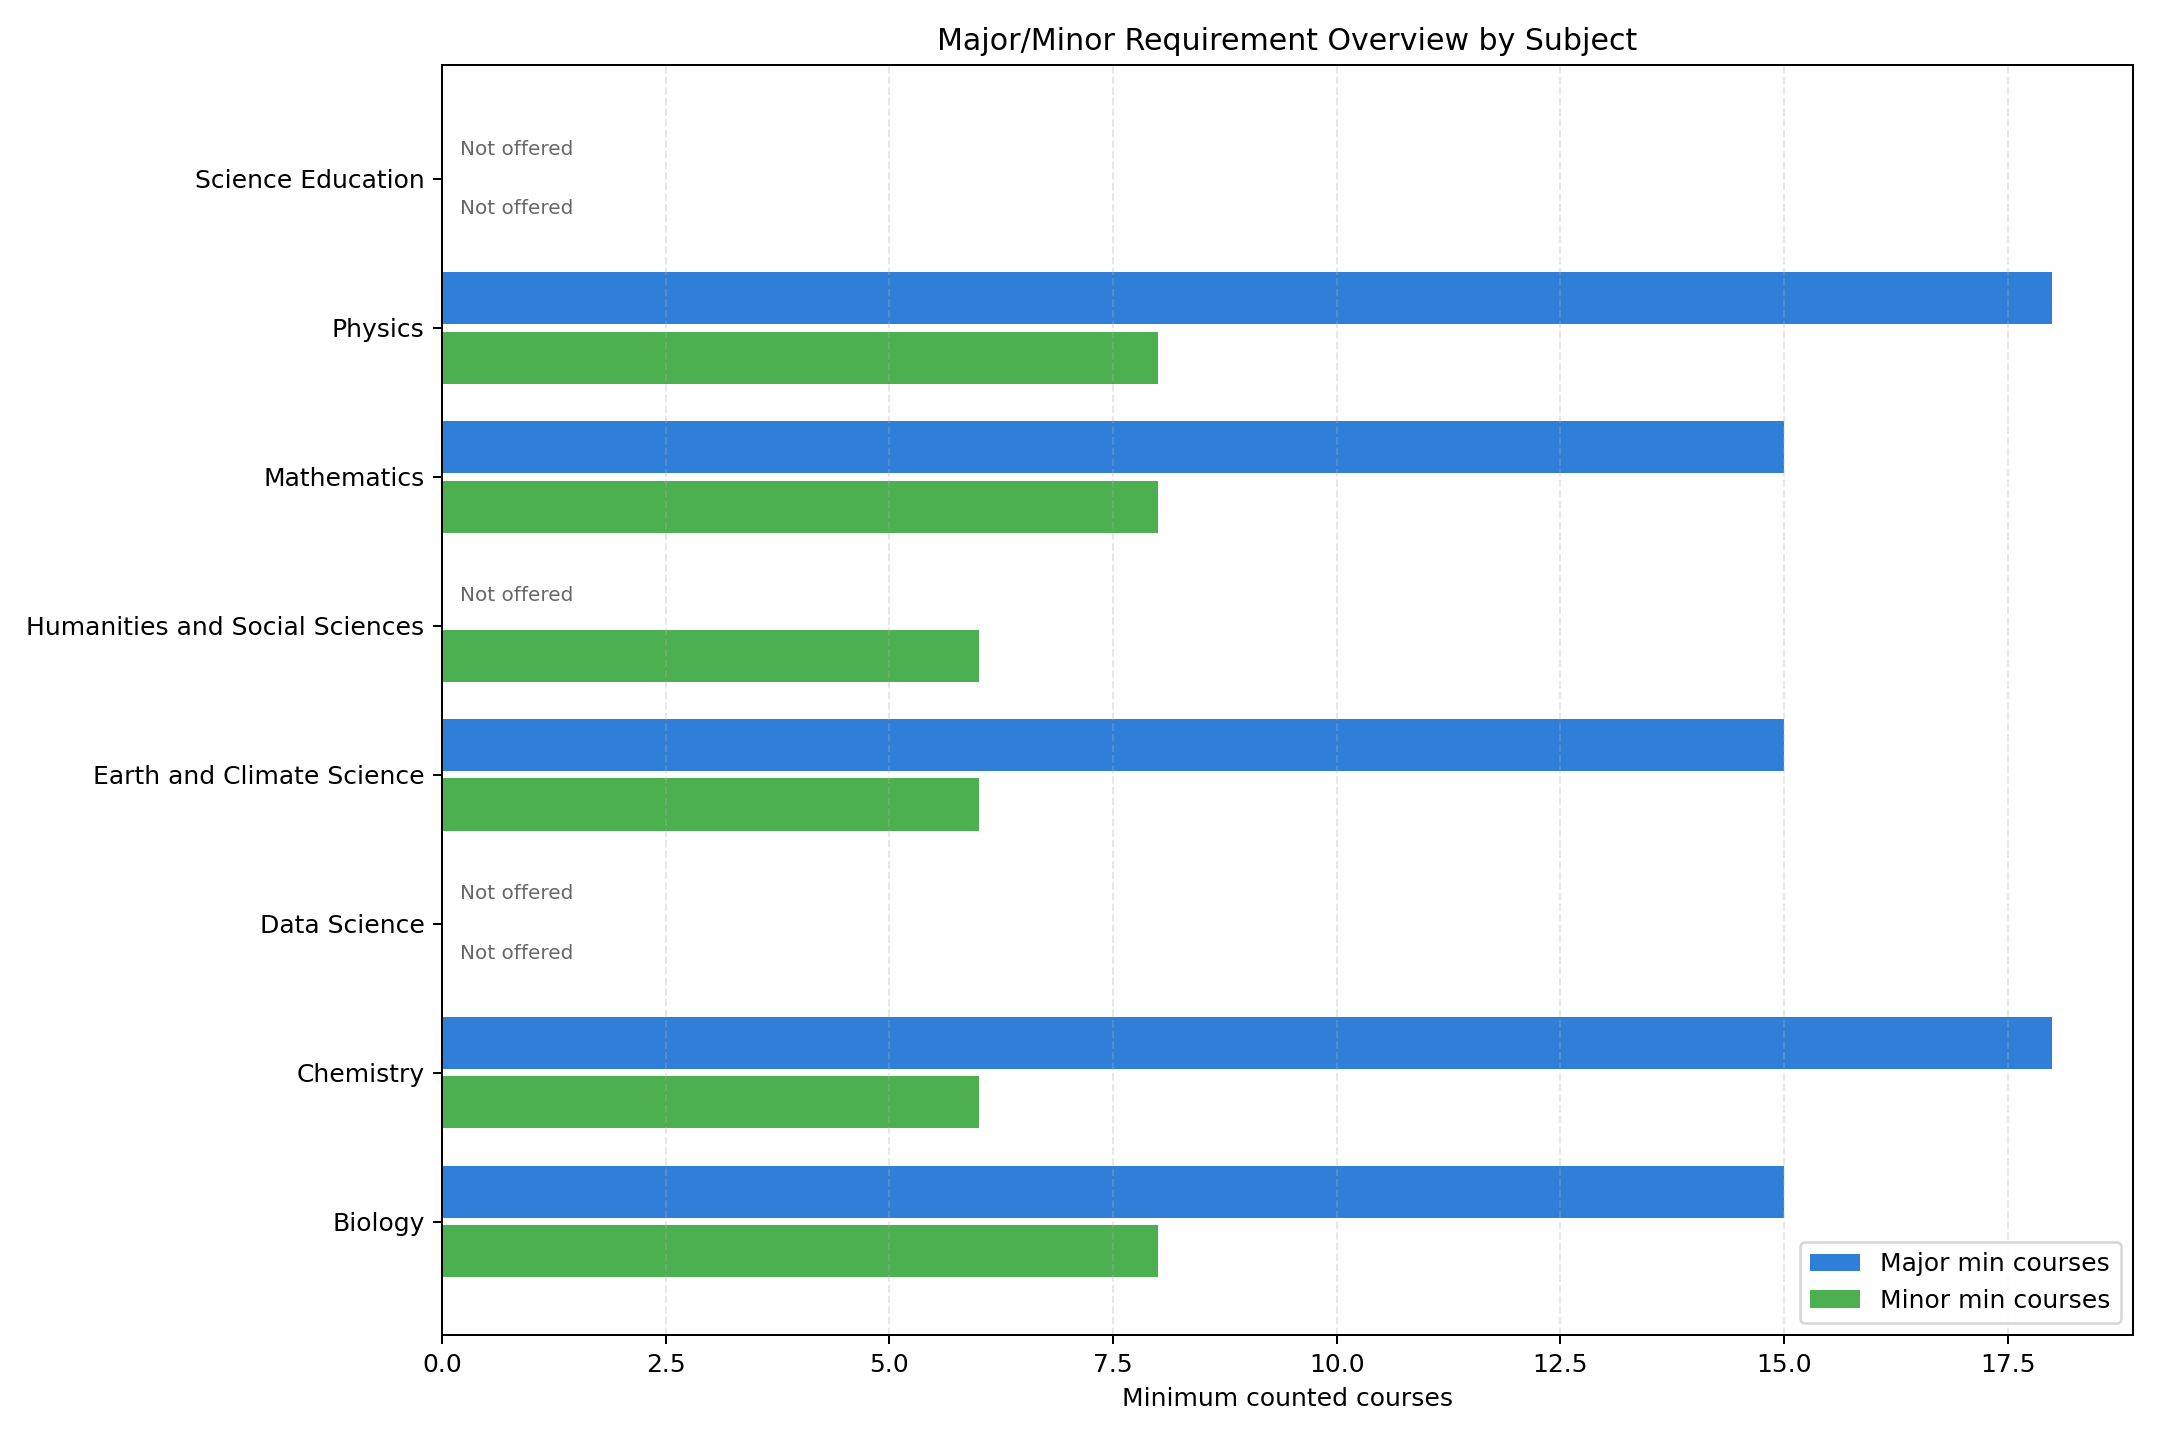
\includegraphics[width=0.92\textwidth]{./figs/major_minor_overview.png}%
    }{%
        \fbox{\parbox[c][0.35\textwidth][c]{0.85\textwidth}{\centering
            Missing figure:\\
            \path{./figs/major_minor_overview.png}
        }}%
    }
    \caption{Overview of major-minor requirement structure used in the planning system.}
    \label{fig:majmin-overview}
\end{figure}

\subsection{Visual Analytics and Plots}
Figure~\ref{fig:sem-year} shows the course distribution by semester and year,
while Fig.~\ref{fig:subject-patterns} shows subject-level and prerequisite
structure patterns.

\begin{figure}[tbp]
    \centering
    \begin{minipage}{0.48\textwidth}
        \centering
        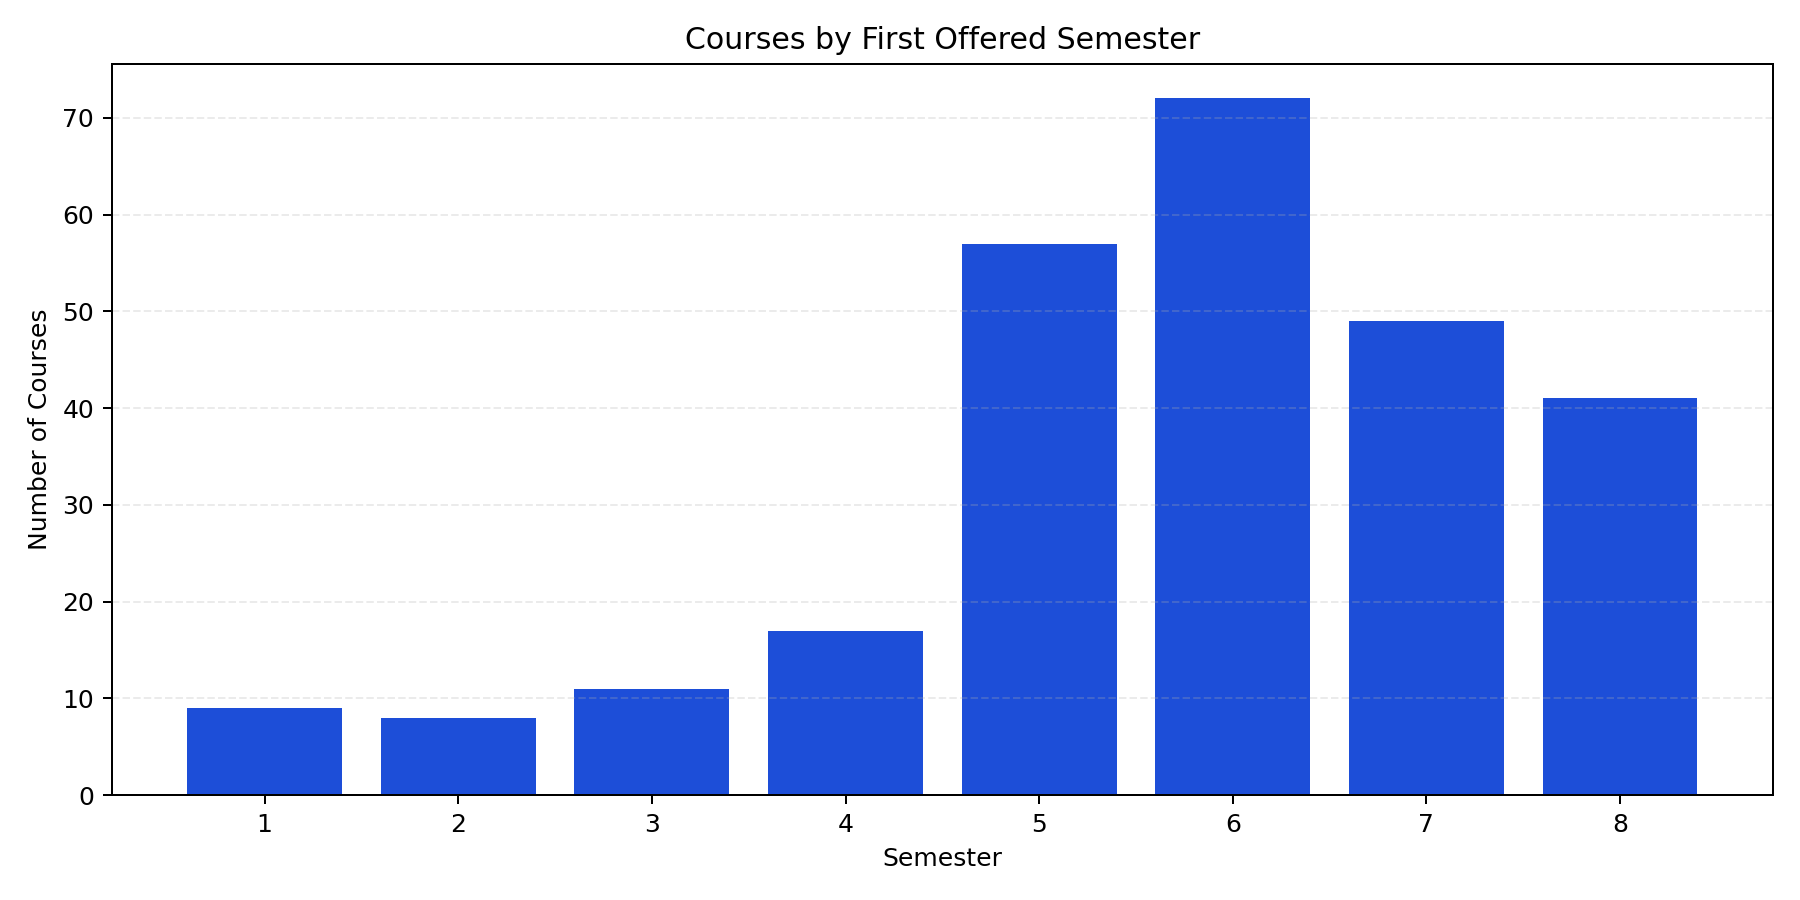
\includegraphics[width=\textwidth]{./figs/courses_by_first_semester.png}
    \end{minipage}
    \hfill
    \begin{minipage}{0.48\textwidth}
        \centering
        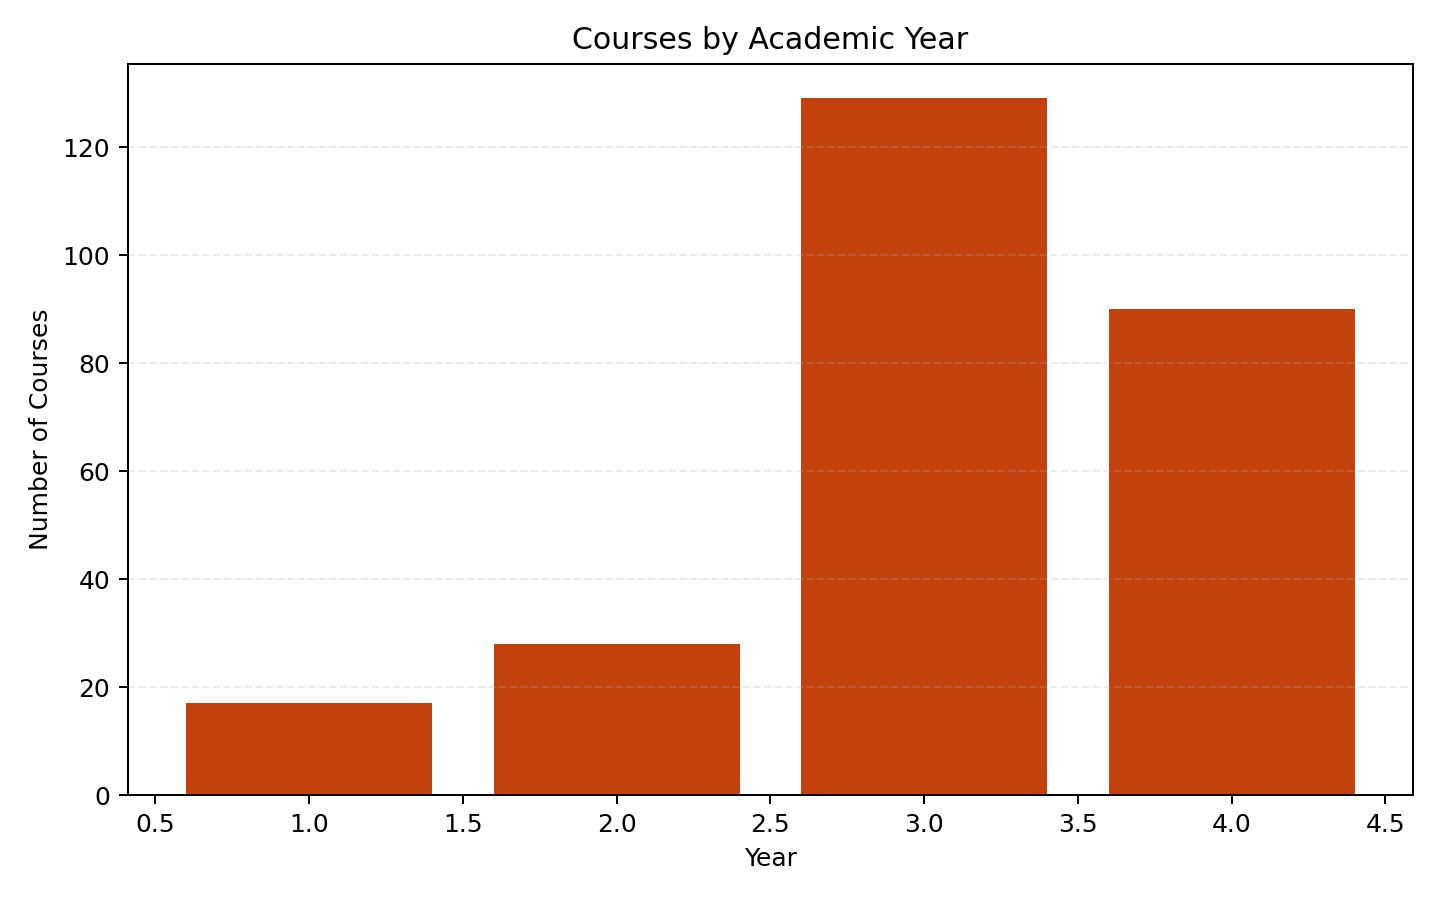
\includegraphics[width=\textwidth]{./figs/courses_by_year.png}
    \end{minipage}
    \caption{Course availability distribution over semester and academic year.}
    \label{fig:sem-year}
\end{figure}

\begin{figure}[tbp]
    \centering
    \begin{minipage}{0.48\textwidth}
        \centering
        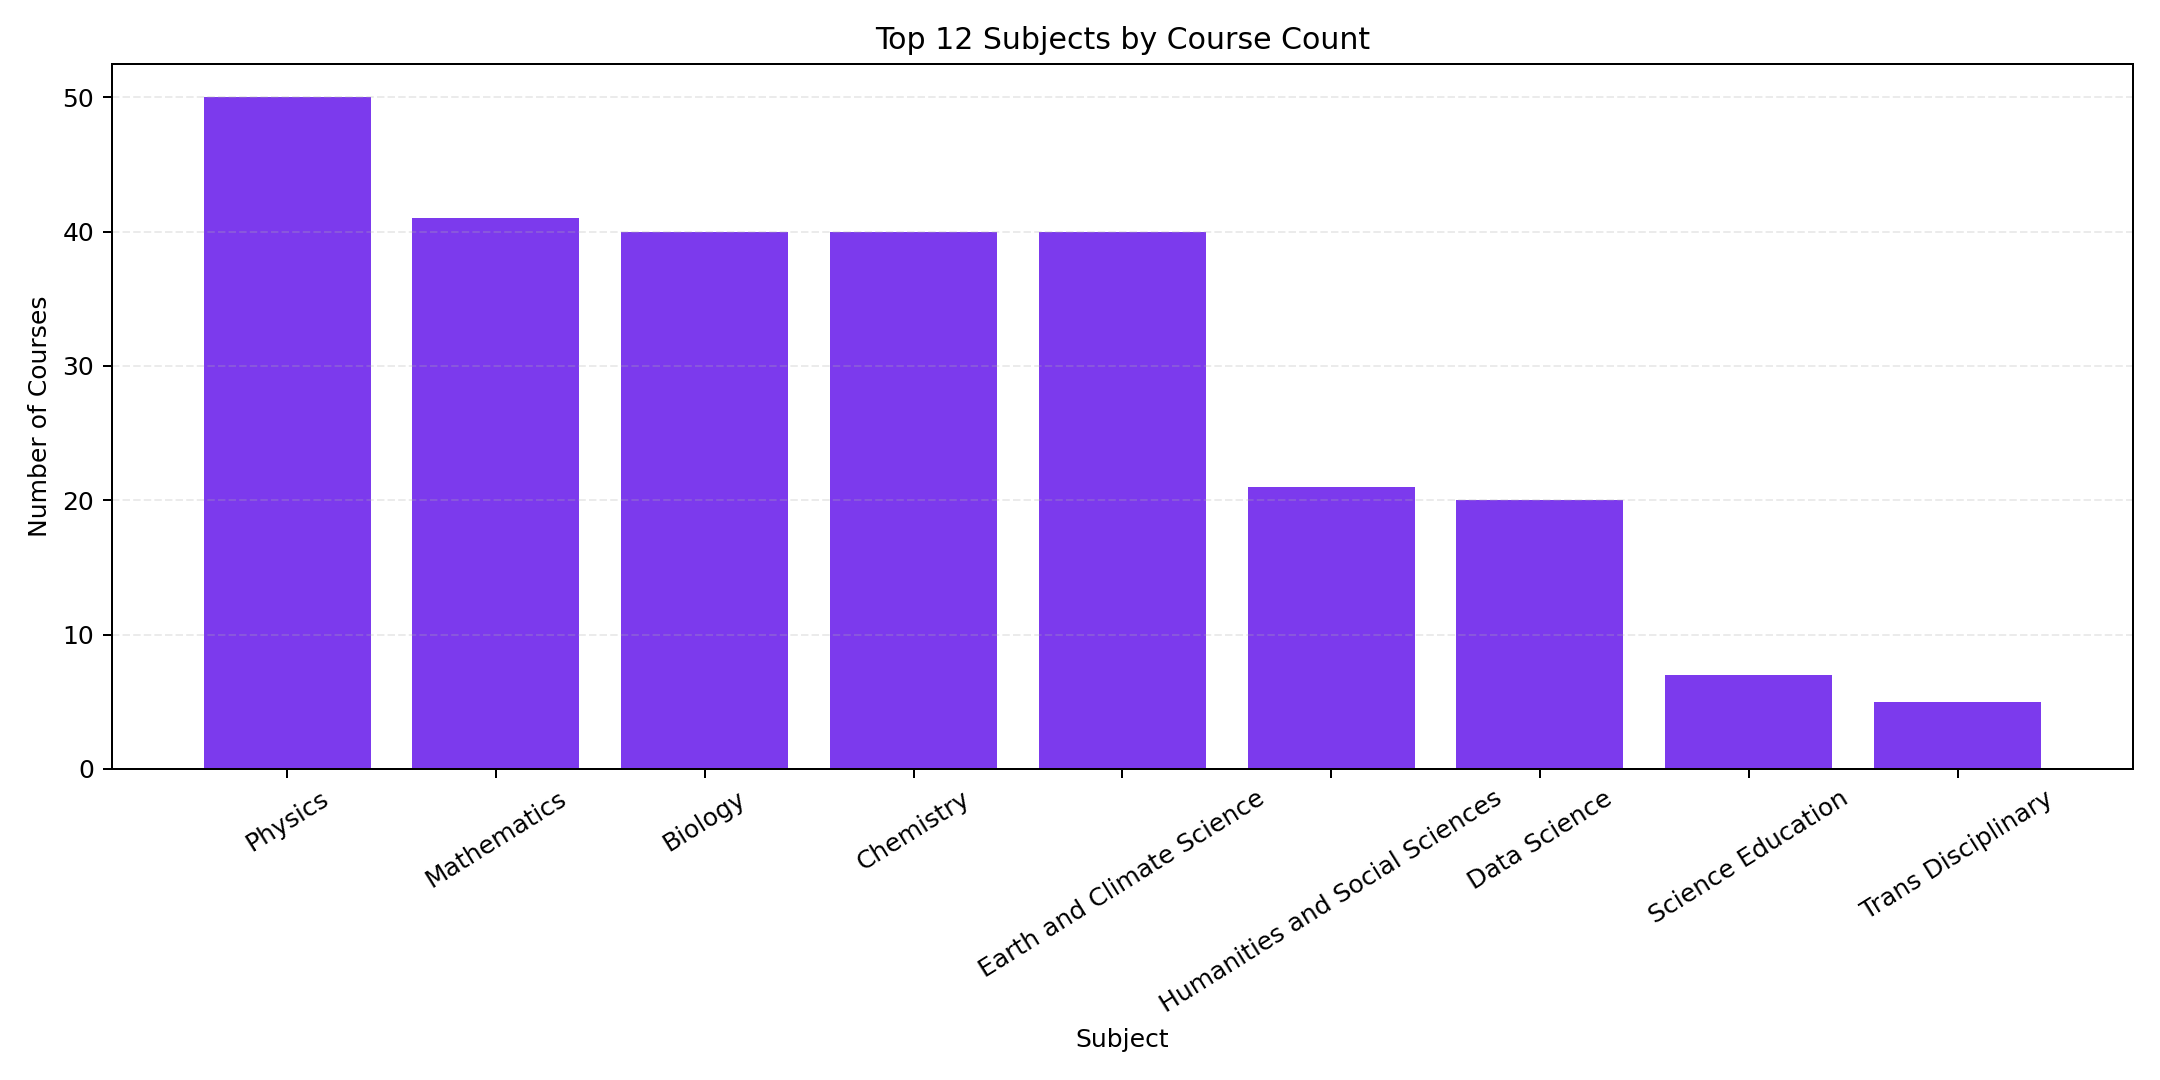
\includegraphics[width=\textwidth]{./figs/subject_distribution_top.png}
    \end{minipage}
    \hfill
    \begin{minipage}{0.48\textwidth}
        \centering
        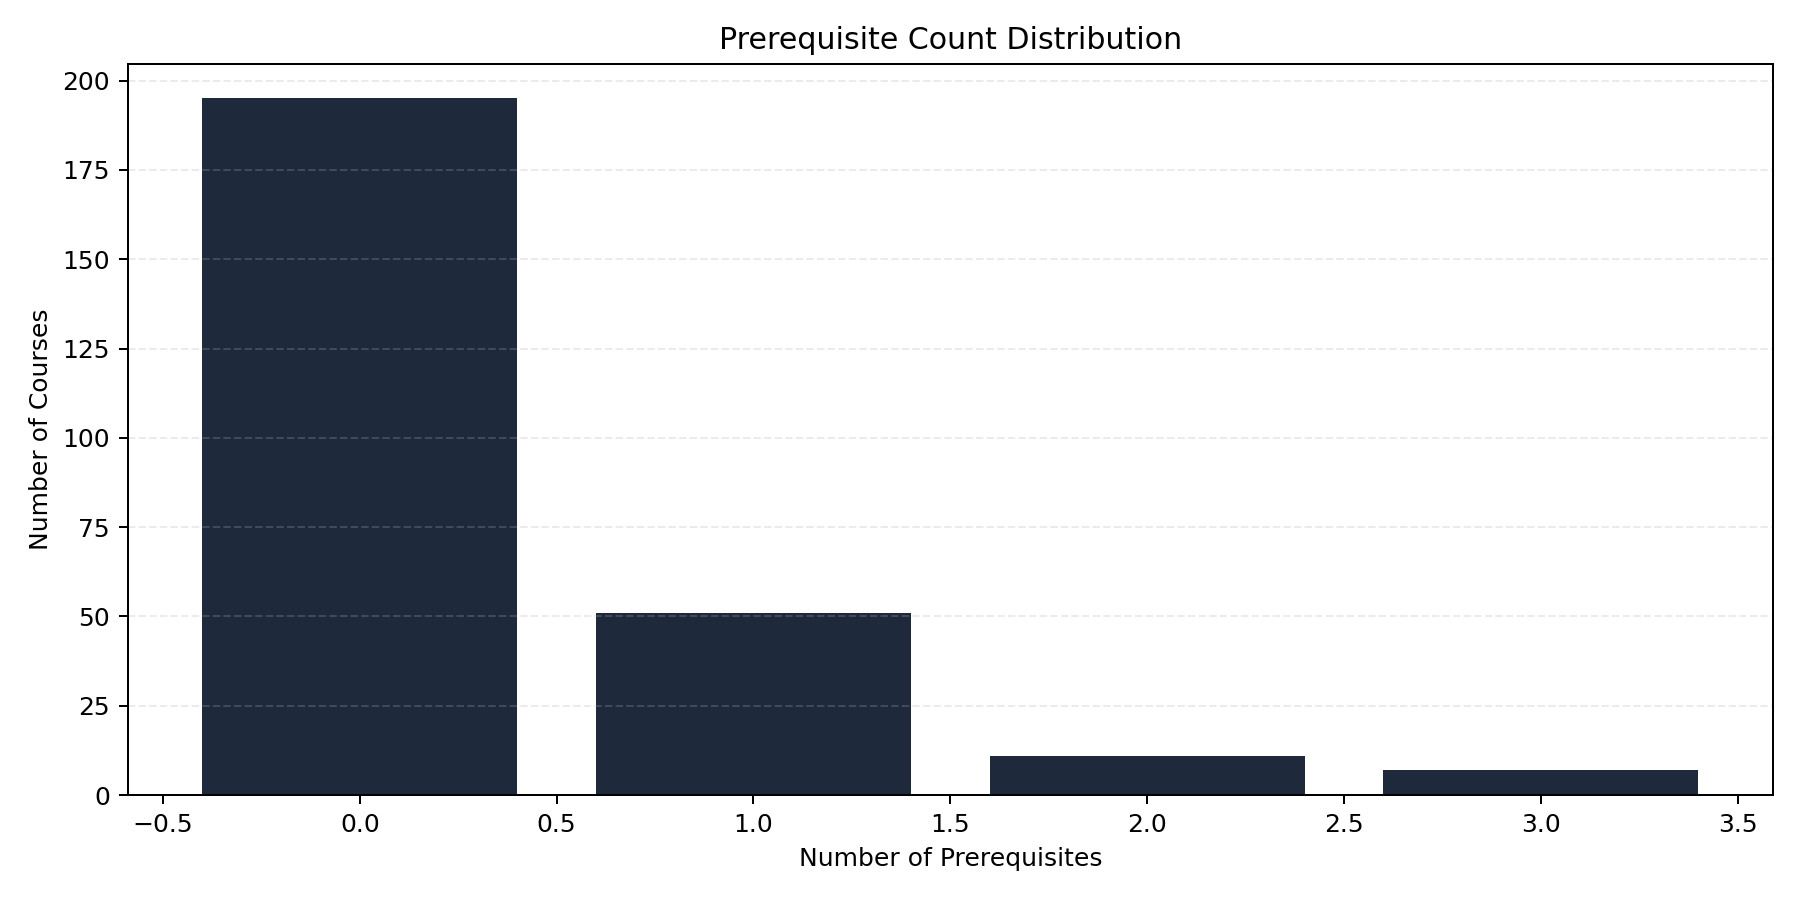
\includegraphics[width=\textwidth]{./figs/prerequisite_count_distribution.png}
    \end{minipage}
    \caption{Subject concentration and prerequisite count structure.}
    \label{fig:subject-patterns}
\end{figure}

\subsection{Dashboard}

The primary output is a Streamlit server featuring an interactive graph display. The UI allows users to:
\begin{itemize}
    \item Visualize all courses with prerequisites, grouped by semester.
    \item Set interactive options for major, minor, and personal preferences.
    \item View all valid pathways based on the options chosen by the user.
\end{itemize}

\subsection{USe Case}

A student can use this tool to set a major and minor and other preferences. 
They can view exactly which prerequisites are required and how they fit into their existing corses. 
The system ensures that credit limits per semester are not exceeded.

\section{Conclusion and Outlook}

The Curriculum Graph system provides an interactive solution for academic planning. 
By representing dependencies as a directed acyclic graph, 
it offers students a clear, customizable roadmap to finish their degree requirements.

\section{Acknowledgements}
We acknowledge the course and program-rule data sources provided for IISER Pune
curriculum modeling, and the open-source tools that enabled this work.

\section{Author Contributions}

The project responsibilities were distributed as follows:
\begin{itemize}
    \item \textbf{Ayush Raj}: Data Validation, Graph Construction, and UI Testing.
    \item \textbf{Applen Tahu}: Data Extraction, JSON Schema design, and UI Design.
    \item \textbf{Malhar Patel}: Graph Algorithms and UI Construction.
    \item \textbf{Sankar Maharajan}: Data Preprocessing and Graph Validation.
\end{itemize}

\section{Code availability}
Source code (GitHub): \url{https://github.com/Mal-Pat/curriculum-graph}.

% --------------------------------------------------------------------
% --------------------------------------------------------------------
% ---- DO NOT CHANGE THIS BLOCK OF CODE
\section{References}
\bibliography{refs}
% --------------------------------------------------------------------
% --------------------------------------------------------------------


% --------------------------------------------------------------------
% --------------------------------------------------------------------
% ---- DO NOT CHANGE THIS BLOCK OF CODE
\end{document}
% --------------------------------------------------------------------
% --------------------------------------------------------------------
